\chapter{CÔNG THỨC TOÁN HỌC}

\section{Entropy}
Entropy là thuật ngữ thuộc Nhiệt động lực học, là thước đo của sự biến đổi,
hỗn loạn hoặc ngẫu nhiên.
Năm 1948, Shannon đã mở rộng khái niệm Entropy sang lĩnh vực nghiên cứu,
thống kê với công thức như sau:

Với một phân phối xác suất của một biến rời rạc $x$ có thể nhận $n$ giá trị
khác nhau $x_1, x_2,..., x_n$

Giả sử rằng xác suất để $x$ nhận các giá trị này là $p_i=p(x=x_i)$.

Ký hiệu phân phối này là $p=(p_1, p_2,..., p_n)$.
Entropy của phân phối này được định nghĩa là:

\begin{equation*}
    H(p)=-\sum_{n=1}^{n}p_ilog(p_i)
\end{equation*}

trong đó $log$ là logarit tự nhiên
(Một số tài liệu dùng logarit cơ số 2, nhưng giá trị của $H(p)$
chỉ khác đi bằng cách nhân với một hằng số.) và quy ước $0log(0)=0$

Giả sử bạn tung một đồng xu, Entropy sẽ được tính như sau:

\begin{equation*}
    H = -[0.5log(0.5) + 0.5log(0.5)]
\end{equation*}

\begin{center}
    \begin{figure}[ht!]
        \begin{center}
         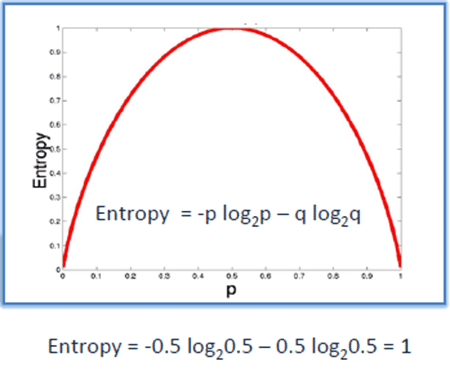
\includegraphics[scale=0.7]{thesis/decision-tree/mathematical/dt_ex2.png}
        \end{center}
        \caption{Hàm Entropy.}
        \label{fig:dt_ex2}
    \end{figure}
\end{center}

Hình vẽ trên biểu diễn sự thay đổi của hàm Entropy.
Ta có thể thấy rằng, Entropy đạt tối đa khi xác suất xảy ra của hai lớp bằng nhau.

\begin{itemize}
    \item P tinh khiết: $p_i=0$ hoặc $p_i=1$
    \item P vẩn đục: $p_i=0.5$, khi đó hàm Entropy đạt đỉnh cao nhất
\end{itemize}

Entropy trong học máy và lý thuyết thông tin nói chung là thước đo tính ngẫu nhiên
của thông tin đang được xử lý. Entropy càng cao, càng khó rút ra bất kỳ kết luận nào
từ thông tin đó.
Tung một đồng xu là một ví dụ về thông tin ngẫu nhiên,
trong trường hợp này Entropy đạt cực đại bằng 1,
không có kết luận nào giúp dự đoán được kết quả tung đồng xu.

\section{Information Gain}
Information Gain dựa trên sự giảm của hàm Entropy khi tập dữ liệu được phân chia
trên một thuộc tính. Để xây dựng một Decision Tree, ta phải tìm tất cả thuộc tính
trả về Infomation Gain cao nhất.

Để xác định các nút trong mô hình Decision Tree, ta thực hiện tính
Infomation Gain tại mỗi nút theo trình tự sau:

\begin{itemize}
    \item \textbf{Bước 1:} Tính toán hệ số Entropy của biến mục tiêu $S$ có $N$ phần tử
    với $N_c$ phần tử thuộc lớp $c$ cho trước:
    \begin{equation*}
        H(S) = -\sum_{c=1}^{c}(N_c/N)log(N_c/N)
    \end{equation*}

    \item \textbf{Bước 2:} Tính hàm số Entropy tại mỗi thuộc tính:
    với thuộc tính $x$, các điểm dữ liệu trong $S$ được chia ra $K$
    child node $S_1, S_2,..., S_K$ với số điểm trong mỗi child node
    lần lượt là $m_1, m_2,..., m_K$, ta có:
    \begin{equation*}
        H(x, S) = \sum_{K=1}^{K}(m_K/N)*H(S_K)
    \end{equation*}

    \item \textbf{Bước 3:} Chỉ số Gain Information được tính bằng:
    \begin{equation*}
        G(x, S) = H(S) - H(x, S)
    \end{equation*}
\end{itemize}

\section{Gini Impurity}
Đơn giản hơn so với Entropy và Information Gain, Gini Impurity
là chỉ số thể hiện mức độ phân loại sai khi ta chọn ngẫu nhiên
một phần tử từ tập data. Gini Impurity có công thức như sau:

\begin{equation*}
    G = \sum_{k=1}^{k}p_k*(1-p_k)^2 = 1 - \sum_{k=1}^{k}(p_k)^2
\end{equation*}

Trong đó:
\begin{itemize}
    \item $G$ là giá trị Gini Impurity
    \item $k$ số các lớp có trong tập data
    \item $p_k$ là xác suất mà một phần tử ngẫu nhiên thuộc lớp $k$
\end{itemize}

Giá trị Gini Impurity sau khi chia của mỗi nhóm đều nhỏ hơn so với giá trị ban đầu
=> Sau khi chia nhóm mức độ phân loại sai của hệ thống đã giảm.
Độ giảm của Gini Impurity được gọi là Gini Gain và có công thức tính tương tự
như Information Gain, chỉ khác là ta sẽ sử dụng giá trị Gini Impurity thay vì Entropy:

\begin{equation*}
    GG(Q) = G_O - \sum_{i=1}^{q}\frac{N_i}{N}G_i
\end{equation*}

Cũng tương tự như với khi sử dụng Entropy, Gini Impurity của một Leaf Node
sẽ là 0 và khi training Decision Tree, điều kiện được chọn để chia nhóm
cũng sẽ được chọn sao cho giá trị Gini Gain là lớn nhất.
